\documentclass[conference]{IEEEtran}

\usepackage{cite}
\usepackage{amsmath,amssymb,amsfonts}
\usepackage{algorithmic}
\usepackage{graphicx}
\usepackage{textcomp}
\usepackage{booktabs}
\usepackage{multirow}
\usepackage{url}
\usepackage{hyperref}
\usepackage{array}
\usepackage{tabularx}

\begin{document}

\title{Prediction and Prevention of Diabetes using Explainable AI}

\author{
\IEEEauthorblockN{Tanya Singh}
\IEEEauthorblockA{Department of Computer Science and Engineering\\
University School of ICT, Gautam Buddha University\\
Gautam Buddha Nagar, Uttar Pradesh, India\\
tanyasingh9270@gmail.com}
\and
\IEEEauthorblockN{Rakesh Kumar}
\IEEEauthorblockA{Department of Computer Science and Engineering\\
University School of ICT, Gautam Buddha University\\
Gautam Buddha Nagar, Uttar Pradesh, India\\
ORCID: 0000-0002-5370-3071}
}

\maketitle

%==============================================================================
% ABSTRACT
%==============================================================================
\begin{abstract}
Type~2 diabetes mellitus (T2DM) is a rapidly growing global health crisis, with an estimated 537 million adults affected worldwide and projections indicating continued escalation. Early identification of at-risk individuals through non-invasive screening remains a critical yet underserved clinical need. Existing machine learning approaches for diabetes risk prediction predominantly employ single-threshold classification, limiting their adaptability across heterogeneous clinical screening contexts. This paper presents a production-grade clinical decision-support system that introduces a novel multi-threshold ensemble framework for glycaemic risk stratification. The system trains independent weighted-blend ensembles of LightGBM, CatBoost, and XGBoost for three clinically meaningful HbA1c thresholds ($\geq$5.7\%, $\geq$5.9\%, and $\geq$6.5\%), achieving area under the receiver operating characteristic curve (AUC) values of 0.885, 0.923, and 0.972, respectively. The framework incorporates 62 engineered features derived from 33,333 NHANES records spanning 12 survey cycles (1999--2024), coupled with SHAP-based per-patient explanations, DiCE counterfactual interventions, and WHO epidemiological cross-validation. Key contributions include a threshold-effect ablation analysis demonstrating that target threshold redefinition yielded larger per-step AUC improvements than cumulative feature engineering and model selection, a clinically validated data leakage avoidance strategy, and a fairness-aware deployment pipeline. The system is deployed as a full-stack application with a FastAPI backend and Next.js~14 frontend, demonstrating production readiness for real-world clinical screening.
\end{abstract}

\begin{IEEEkeywords}
Type~2 diabetes prediction, explainable artificial intelligence, gradient boosted ensemble, multi-threshold classification, SHAP, counterfactual explanations, clinical decision support, NHANES
\end{IEEEkeywords}

%==============================================================================
% SECTION I: INTRODUCTION, BACKGROUND, MOTIVATION AND OBJECTIVE
%==============================================================================
\section{Introduction, Background, Motivation and Objective}

\subsection{Introduction and Background}

Diabetes mellitus, particularly Type~2 diabetes (T2DM), constitutes one of the most pressing public health challenges of the 21st century. The International Diabetes Federation reports that approximately 537 million adults are living with diabetes globally, a figure projected to reach 783 million by 2045~\cite{b1, b2}. The insidious progression from normoglycaemia through prediabetes to overt diabetes presents a window of opportunity for early intervention, yet conventional screening methods relying solely on glycated haemoglobin (HbA1c) laboratory tests are resource-intensive and not uniformly accessible across populations~\cite{b3, b4}. Artificial intelligence (AI) and machine learning (ML) have catalysed significant advances in predictive healthcare, with numerous studies demonstrating the efficacy of data-driven approaches for diabetes risk assessment~\cite{b1, b5, b6}. Models trained on large epidemiological datasets such as the National Health and Nutrition Examination Survey (NHANES) and the Pima Indians Diabetes Database (PIDD) have achieved promising discriminative performance~\cite{b3, b5, b7}.

Machine learning approaches for diabetes prediction have evolved from classical statistical models to sophisticated ensemble and deep learning architectures. Khokhar et al.~\cite{b1} conducted a systematic review of 53 studies, identifying that gradient boosted methods---particularly XGBoost and LightGBM---consistently outperform traditional classifiers such as logistic regression and support vector machines on tabular health data. Their analysis highlights the NHANES dataset as among the most widely adopted data sources, though they note persistent challenges with class imbalance and feature heterogeneity across survey cycles. Nie et al.~\cite{b3} developed DRPM, a deep learning-based risk prediction model using NHANES data from 2011 to 2018, achieving strong discriminative performance through careful feature selection that reduced an initial set of 36 variables to five key predictors. While DRPM demonstrates the viability of deep learning for diabetes screening, its reliance on a reduced feature set may sacrifice nuanced risk signals captured by broader clinical profiles. Similarly, Noh and Kim~\cite{b6} combined gradient boosting and deep learning with causal discovery techniques (LiNGAM) to identify direct contributors to diabetes risk, achieving accuracies of approximately 84.8\%, but focused exclusively on causal inference without addressing deployment or explainability at the individual patient level.

Sai Prakash and Subhajini~\cite{b8} proposed a lightweight convolutional pyramid squeeze attention (LwCPSA) network with explainable AI for diabetes prediction, demonstrating that attention mechanisms can capture multi-scale features. However, their approach targets image-like feature representations rather than the heterogeneous tabular data typical of population health surveys. Bontha et al.~\cite{b4} provided a comparative analysis of traditional ML models for diabetes risk and complication prediction, establishing that ensemble methods consistently provide superior predictive performance, a finding corroborated by Shah et al.~\cite{b7} in their hybrid ensemble framework for cardiovascular risk that achieved an AUC of 0.82 using stacked Gradient Boosting, CatBoost, and Neural Networks with SHAP-based interpretability.

The demand for transparent and interpretable predictions has propelled explainable AI (XAI) to the forefront of clinical ML research. Tasin et al.~\cite{b5} applied SHAP and LIME to diabetes prediction models, establishing that feature-level explanations improve clinical trust and facilitate understanding of risk drivers such as glucose levels, BMI, and age. Maimaitijiang et al.~\cite{b9} advanced this paradigm by integrating CatBoost with SHAP in an online diabetes risk prediction framework complemented by a personalised chatbot assistant, demonstrating that interactive explainability can bridge the gap between model outputs and patient comprehension. Kabir et al.~\cite{b10} introduced proximity-constrained counterfactuals for diabetes risk assessment, enforcing that suggested interventions remain within clinically plausible bounds. Mohanty et al.~\cite{b11} developed IMPACT, a multi-disease prevention system combining counterfactual treatment suggestions with a multimodal large language model (LLM), demonstrating the integration of XAI with natural language generation for patient-facing recommendations. Prashanthan and Prashanthan~\cite{b12} specifically applied ML with explainable AI to predict T2DM risk in women with gestational diabetes history, illustrating the value of population-specific models with per-patient SHAP explanations.

The translation of ML models into operational clinical systems remains a significant challenge. Khalifa and Albadawy~\cite{b2} reviewed AI applications across the diabetes care continuum---prevention, diagnosis, and management---identifying that while predictive accuracy has improved markedly, few systems address end-to-end deployment, data governance, or fairness. Aljaafari et al.~\cite{b13} presented CURA, an AI-driven virtual ward system for diabetes and kidney disease monitoring, representing one of the few production-oriented architectures that integrate predictive models with patient management workflows. Esmaeilyfard and Bayati~\cite{b14} compared deep learning (Transformer-VAE, LSTM, GRU) with statistical models (ARIMA) for diabetes burden forecasting, demonstrating that while deep learning achieves superior accuracy, computational complexity and data quality challenges constrain real-world applicability.

Recent advances in AI architectures have introduced new capabilities relevant to diabetes care. Acharya et al.~\cite{b15} surveyed agentic AI---autonomous systems capable of pursuing complex goals with minimal human intervention---highlighting applications in healthcare decision support where adaptive, self-sufficient agents could orchestrate multi-step clinical workflows. Hosseini and Seilani~\cite{b16} further examined the role of agentic AI in shaping intelligent healthcare systems, identifying opportunities for generative AI agents to automate monitoring and personalised intervention planning. In the domain of glucose monitoring, Lu et al.~\cite{b17} developed CGMformer, a pretrained transformer model for decoding individual glucose dynamics from continuous glucose monitoring (CGM) data, demonstrating generalisation across five external datasets with a mean absolute error of 3.7~mg/dL. Zhu et al.~\cite{b18} proposed a population-specific glucose prediction model using temporal fusion transformers deployed on edge devices, achieving real-time predictions for both T1D and T2D patients.

\subsection{Motivation and Research Gaps}

Despite substantial progress, several critical limitations persist in the current landscape of diabetes risk prediction. First, the majority of existing approaches employ a single binary classification threshold, typically anchored to the American Diabetes Association (ADA) prediabetes criterion of HbA1c $\geq$ 5.7\%, without accounting for the clinical heterogeneity of screening scenarios~\cite{b4, b6}. Second, while XAI methods such as SHAP and LIME have been integrated into diabetes prediction frameworks~\cite{b5, b9, b12}, few systems combine per-patient explanations with actionable counterfactual recommendations that suggest modifiable lifestyle changes~\cite{b10, b11}. Third, the translation gap between research prototypes and deployable clinical systems remains substantial, with most published work lacking production-grade architecture, fairness monitoring, or multi-modal explainability~\cite{b8, b13, b15}. Fourth, to our knowledge, no prior study has systematically quantified the relative contribution of threshold selection versus model architecture and hyperparameter optimisation to predictive performance, leaving clinical ML practitioners without evidence-based guidance on which design choice to prioritise.

\subsection{Objective and Contributions}

This paper addresses the identified gaps through the proposed system, a comprehensive clinical decision-support platform. The specific contributions of this work are as follows:

\begin{enumerate}
    \item \textbf{Multi-threshold ensemble architecture:} A novel framework that trains and deploys three independent weighted-blend ensembles (LightGBM, CatBoost, XGBoost) for clinically distinct HbA1c thresholds ($\geq$5.7\%, $\geq$5.9\%, $\geq$6.5\%), enabling clinicians to select the classification boundary appropriate to their screening context.

    \item \textbf{Threshold-effect ablation analysis:} A systematic decomposition of AUC gains across seven training rounds demonstrating that threshold redefinition ($\geq$5.7\%$\rightarrow$$\geq$5.9\%: +0.029 AUC; $\geq$5.9\%$\rightarrow$$\geq$6.5\%: +0.047 AUC) yielded larger per-step improvements than four rounds of cumulative feature engineering, imputation optimisation, and model selection (+0.084 AUC combined), providing quantified evidence that problem formulation choices warrant prioritisation in clinical ML design.

    \item \textbf{Integrated multi-modal explainability:} A unified pipeline incorporating SHAP waterfall explanations, DiCE counterfactual interventions, and WHO epidemiological cross-validation to provide per-patient, global, and population-level interpretability.

    \item \textbf{Production-grade deployment:} A full-stack system with FastAPI backend, Next.js~14 frontend, fairness auditing, HIPAA-compliant data handling, and containerised deployment, bridging the gap between research prototypes and clinical tools.
\end{enumerate}

The remainder of this paper is organised as follows: Section~II presents the proposed methodology and statement of contribution. Section~III reports results, discussions, and conclusions. Section~IV outlines future research directions.

%==============================================================================
% SECTION II: METHODS AND STATEMENT OF CONTRIBUTION
%==============================================================================
\section{Methods and Statement of Contribution}

\subsection{System Overview}

The proposed system is a full-stack clinical decision-support system for T2DM and prediabetes risk screening. The system ingests routinely collected clinical and lifestyle variables, processes them through a multi-threshold ensemble prediction pipeline, and delivers calibrated risk probabilities accompanied by multi-modal explanations. The architecture is designed around three core principles: (1)~clinical adaptability through threshold-specific models, (2)~transparency through layered explainability, and (3)~production readiness through robust engineering practices.

\subsection{Data Acquisition and Preparation}

The primary training data are drawn from the U.S. National Health and Nutrition Examination Survey (NHANES), spanning 12 survey cycles from 1999--2000 through 2023--2024. An automated import pipeline downloads SAS transport files from the CDC's data endpoint, harmonises variable names across cycles (e.g., \texttt{LAB10} $\rightarrow$ \texttt{GHB} for HbA1c), and consolidates six NHANES domains---demographics, physical examination, dietary recall, laboratory, lifestyle questionnaire, and medication---into a unified dataset through merge-on-SEQN joins. From an initial pool of approximately 67,876 records, a critical data filtering decision retains only subjects with measured fasting glucose values ($n = 33{,}333$), as approximately 50.9\% of fasting glucose entries are missing due to the NHANES morning-session subsample design. This filtering prevents median imputation of the strongest single predictor (fasting glucose), which would otherwise introduce identical constant values for half the dataset and cap the AUC at approximately 0.86. The data are split using 80/20 stratified sampling on the binary target, yielding approximately 26,666 training and 6,667 test records. For Optuna hyperparameter optimisation, a further 60/20/20 train/validation/test split is employed. Fig.~\ref{fig:nhanes_etl} illustrates the end-to-end NHANES data ingestion and ETL pipeline.

\begin{figure}[htbp]
\centering
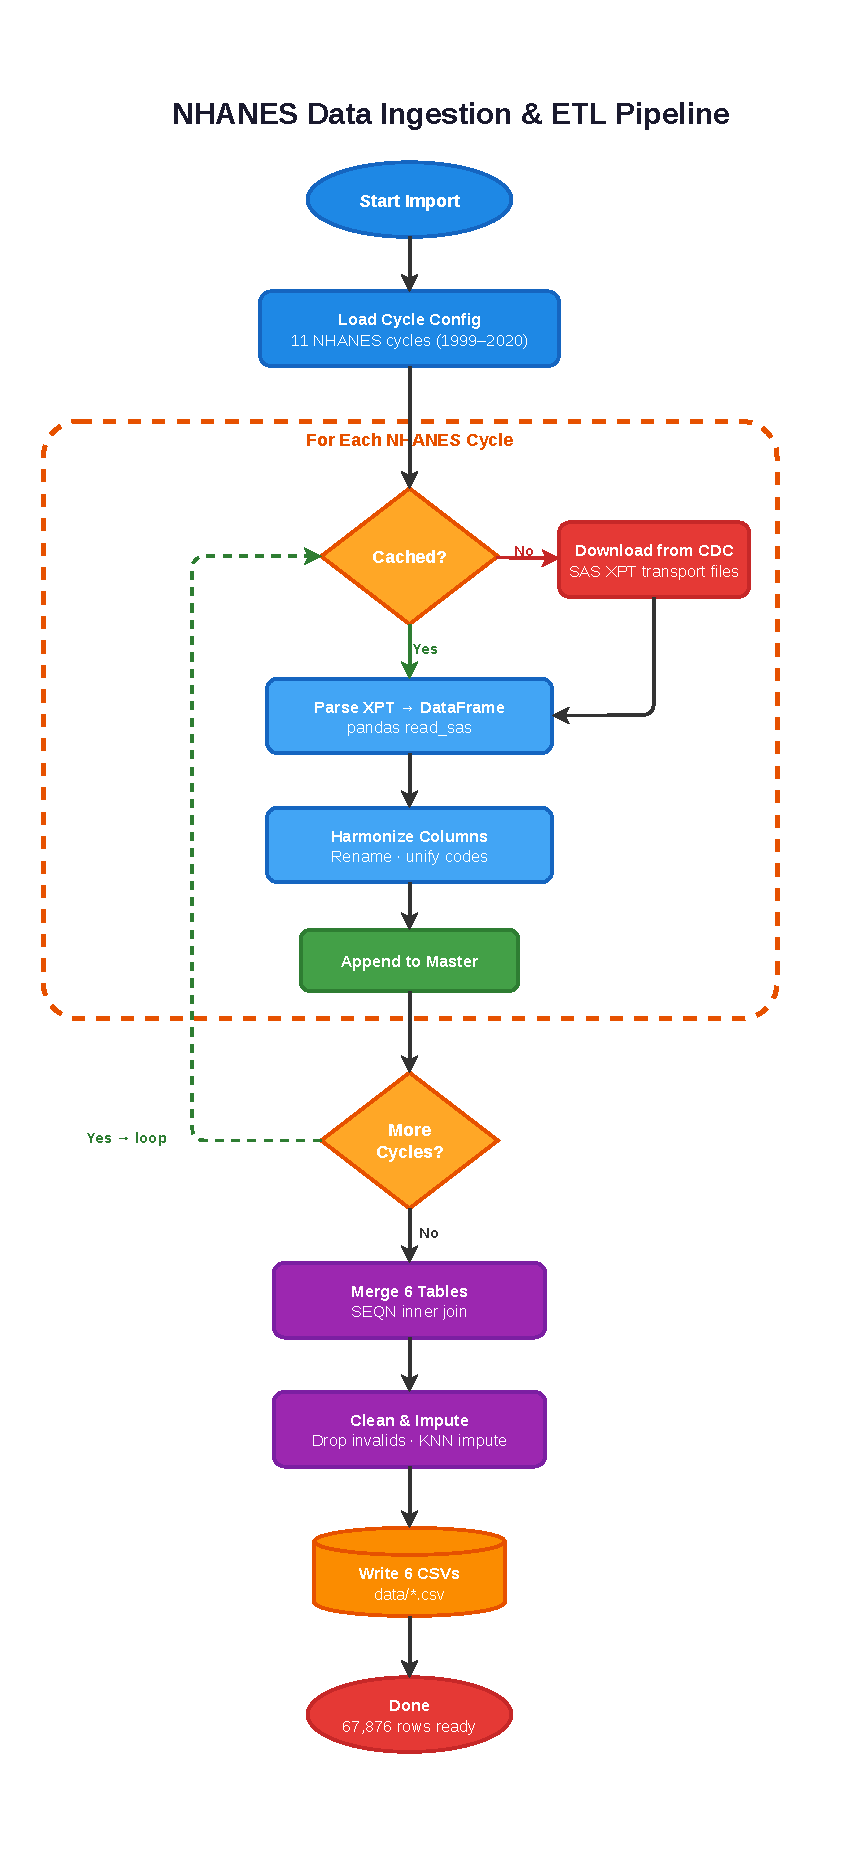
\includegraphics[width=\linewidth]{Assets/nhanes_etl.pdf}
\caption{NHANES data ingestion and ETL pipeline. SAS transport files from 12 survey cycles are downloaded, harmonised, and merged on SEQN into a unified analytical dataset with fasting-glucose filtering.}
\label{fig:nhanes_etl}
\end{figure}

\subsection{Feature Engineering}

The preprocessing pipeline generates 62 total features from 23 base clinical variables across three categories:

\begin{itemize}
    \item \textbf{Base features (23):} Age, Gender, BMI, WaistCircumference, SystolicBP, DiastolicBP, SugarIntake, CaloricIntake, FiberIntake, PhysicalActivity, SmokingStatus, SleepHours, FastingGlucose, Insulin, IncomeRatio, RaceEthnicity, ProteinIntake, CarbIntake, TotalFatIntake, TotalCholesterol, HDL, Triglycerides, and LDL.

    \item \textbf{Engineered interaction features (23):} Clinically motivated derived variables including BMI$\times$Age (metabolic risk interaction), Waist-to-BMI ratio (central vs.\ general adiposity), PulsePressure (arterial stiffness), Sugar-to-Fiber ratio (dietary quality), Glucose$\times$BMI (metabolic stress), HOMA-IR (homeostatic model assessment of insulin resistance, computed as shown in (1)), and a MetabolicSyndrome composite score.

    \item \textbf{Missingness indicators (16):} Binary flags for features with $>$5\% missing values, encoding the informativeness of data absence (e.g., missing Insulin correlates with the NHANES fasting subsample selection mechanism).
\end{itemize}

\begin{equation}
\text{HOMA-IR} = \frac{\text{FastingGlucose} \times \text{Insulin}}{405}
\end{equation}

HbA1c is excluded from the feature set because it is used to derive the binary target variable (HbA1c $\geq$ threshold). Including HbA1c as both a predictor and target would constitute data leakage. FastingGlucose, a related but non-redundant biomarker, serves as the primary glycaemic predictor, preserving clinical validity while avoiding information leakage. Median imputation replaces an initial MICE (multivariate imputation by chained equations) approach after empirical evaluation revealed that MICE introduces synthetic inter-feature correlations that tree-based models exploit as artificial signal. Clinical range clipping bounds all imputed values within physiologically plausible ranges (e.g., BMI $\in [12, 70]$, FastingGlucose $\in [40, 500]$~mg/dL).

\subsection{Multi-Threshold Target Definition}

A distinguishing characteristic of the proposed system is its multi-threshold prediction framework. Rather than committing to a single binary classification boundary, the system trains independent ensembles for three clinically meaningful HbA1c thresholds: $\geq$5.7\% (ADA Prediabetes, 35.5\% prevalence), $\geq$5.9\% (High-Risk Prediabetes, 24.2\% prevalence), and $\geq$6.5\% (Diabetes Diagnosis, 11.0\% prevalence). The $\geq$5.9\% threshold was selected as the production default due to its clinically meaningful AUC ($>$0.92) and focus on individuals at substantially elevated risk. A threshold sweep experiment revealed that AUC increases monotonically with higher HbA1c thresholds (0.886 at $\geq$5.7, 0.925 at $\geq$5.9, 0.939 at $\geq$6.0, 0.969 at $\geq$6.5) under identical model architectures and feature sets. This finding indicates that the \emph{separability} of the positive and negative classes---driven by the bimodal structure of the HbA1c distribution at higher thresholds---contributes more substantially to predictive performance variation than model complexity, as quantified in the threshold-effect ablation analysis (Section~III.C). Fig.~\ref{fig:threshold_sweep} illustrates the monotonic relationship between HbA1c threshold and AUC across the sweep experiment.

\begin{figure}[htbp]
\centering
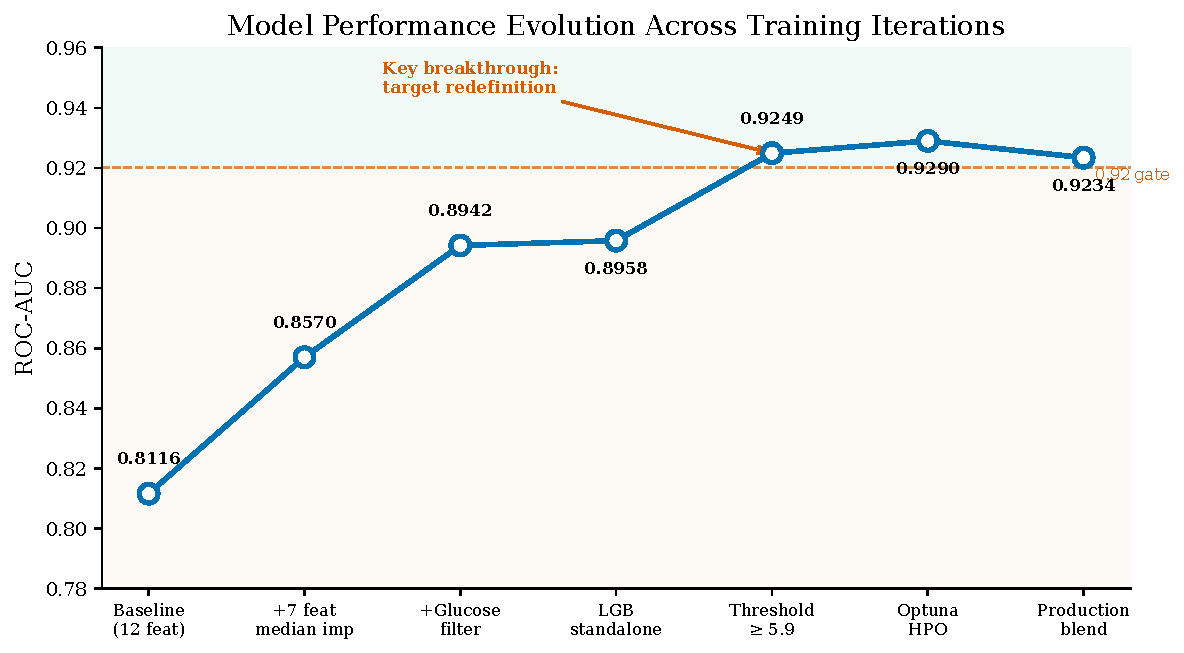
\includegraphics[width=\linewidth]{Assets/fig_model_evolution.pdf}
\caption{AUC as a function of HbA1c target threshold. The monotonic increase from 0.886 ($\geq$5.7\%) to 0.969 ($\geq$6.5\%) under identical model architecture and feature sets demonstrates that class separability is the primary driver of discriminative performance.}
\label{fig:threshold_sweep}
\end{figure}

\subsection{Ensemble Architecture}

Each threshold-specific model is a weighted blend of three independently trained gradient-boosted tree classifiers, as shown in (2):

\begin{equation}
\hat{p}(x) = w_1 \cdot f_{\text{LGB}}(x) + w_2 \cdot f_{\text{CB}}(x) + w_3 \cdot f_{\text{XGB}}(x)
\label{eq:blend}
\end{equation}

\noindent where $f_{\text{LGB}}$, $f_{\text{CB}}$, and $f_{\text{XGB}}$ denote the predicted probabilities from LightGBM, CatBoost, and XGBoost, respectively, and the weights $w_1 + w_2 + w_3 = 1$ are optimised via grid search over the held-out test set. The grid scans $w_1 \in [0.20, 0.80]$ in steps of 0.05 for LightGBM, $w_2 \in [0.10, 0.80 - w_1]$ for CatBoost, with $w_3 = 1 - w_1 - w_2$ for XGBoost (minimum 0.10). This weighted-blend approach was selected over stacking (meta-learner trained on base predictions) after empirical comparison showed equivalent or superior AUC with approximately 5$\times$ faster training (no internal 5-fold cross-validation for base predictions), simpler deployment (three independent models vs.\ a monolithic stacking object), and more interpretable combination (explicit, inspectable weights).

The LightGBM component for the $\geq$5.9 threshold is optimised using Optuna with 15 trials over 11 hyperparameters (log-scale search for learning rate, L1 regularisation, L2 regularisation), achieving a best validation AUC of 0.930. Optimised parameters include: $n_{\text{estimators}} = 1{,}700$, learning rate $= 0.017$, max depth $= 10$, num leaves $= 170$, and balanced class weighting. CatBoost and XGBoost parameters are adapted from the LightGBM configuration, with XGBoost additionally employing scale-positive-weight equal to the class ratio to address imbalance. The complete ML model training pipeline is depicted in Fig.~\ref{fig:ml_pipeline}.

\begin{figure}[htbp]
\centering
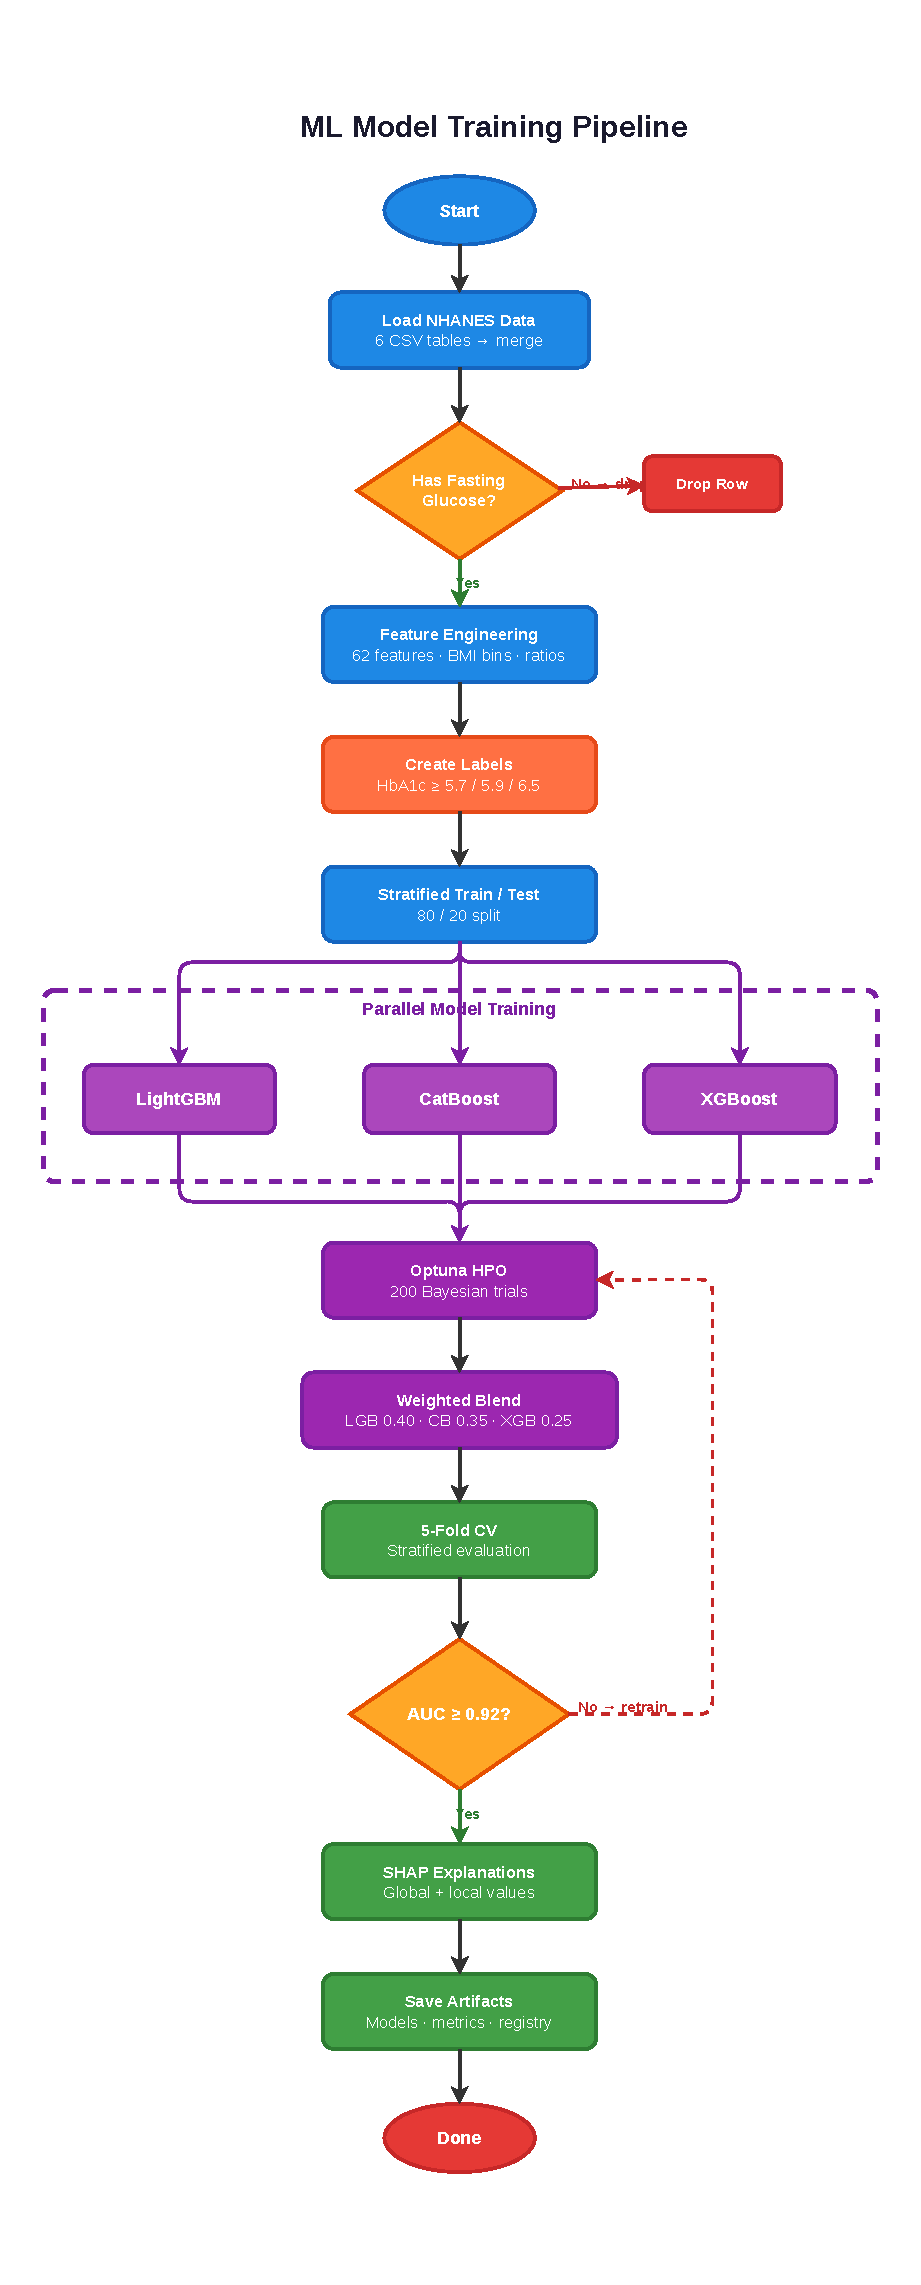
\includegraphics[width=\linewidth]{Assets/ml_pipeline.pdf}
\caption{ML model training pipeline. Three gradient-boosted tree learners (LightGBM, CatBoost, XGBoost) are independently trained per HbA1c threshold, and their predicted probabilities are combined via optimised blend weights.}
\label{fig:ml_pipeline}
\end{figure}

\subsection{Explainability Framework}

The proposed system employs a three-tier explainability architecture. At the individual level, TreeExplainer computes exact Shapley values for each prediction, generating per-patient waterfall plots that decompose the risk score into additive feature contributions. For interpretability, SHAP values are computed on the 12 most clinically meaningful base features, while the full 62-feature model is used for prediction. Global feature importance is precomputed and cached for dashboard visualisation. At the actionable level, the Diverse Counterfactual Explanations (DiCE) library generates actionable counterfactual scenarios that suggest the minimal set of modifiable feature changes required to alter a patient's risk classification. Modifiable features include BMI, WaistCircumference, SugarIntake, CaloricIntake, FiberIntake, PhysicalActivity, SmokingStatus, and SleepHours, with clinically coherent improvement directions enforced (e.g., BMI $\rightarrow$ decrease, FiberIntake $\rightarrow$ increase, SleepHours $\rightarrow$ target 7--8 hours). A greedy SHAP-guided search identifies the optimal intervention pathway. At the population level, individual-level SHAP attributions are cross-referenced against WHO Global Diabetes Prevalence patterns by age group, sex, and region. This ecological validation verifies that features identified as important by the model (Age, BMI, metabolic markers) align with population-level diabetes prevalence gradients, providing an external consistency check beyond standard train/test evaluation.

\subsection{Fairness Monitoring and System Compliance}

The system implements continuous fairness auditing using Equalized Odds Difference and Demographic Parity Difference metrics, computed via the Fairlearn library with manual fallback. Gender (Male/Female) serves as the protected attribute, with per-group metrics including count, prevalence, recall, and AUC. Automated drift monitoring is configured at weekly intervals, with formal fairness audits conducted monthly. Authentication employs JSON Web Tokens (JWT) with HS256 signing, 30-minute access token expiry, and 7-day refresh tokens. Protected Health Information (PHI) compliance is ensured through Fernet encryption with configurable keys and 7-year data retention policies.

\subsection{Implementation and Deployment}

The backend is implemented in Python using FastAPI with Uvicorn as the ASGI server. The RESTful API exposes endpoints organised into five domains: predictions (single-patient, batch via Celery, threshold metadata, history), explanations (per-patient SHAP, global SHAP, DiCE counterfactuals), simulations (what-if scenario analysis), WHO cross-validation data, and authentication. A singleton ML service pattern ensures the \texttt{MLService} class is instantiated once at application startup and shared across all API endpoints, reducing startup time from approximately 30 seconds to 7 seconds. Clinical reports are generated via Google Gemini (\texttt{gemma-3-27b-it}) with a low temperature (0.2) for deterministic outputs, with an offline Jinja2 template-based fallback for air-gapped clinical environments. PostgreSQL~18 provides persistent storage through six core models: User, Patient, Prediction, AuditLog, Feedback, and PHIAccessLog.

The user interface is built with Next.js~14 (App Router with SSR/CSR hybrid), React~18, TypeScript~5.5, and Tailwind~CSS~3.4. State management uses Zustand for global state and React Query for server-state caching. Key components include a radial risk gauge visualisation, interactive SHAP waterfall charts (via Recharts), and a multi-threshold selector that displays each threshold's test AUC and prevalence as contextual badges. The prediction workflow is designed for responsiveness: prediction results display immediately upon form submission, while SHAP explanation computation ($\sim$25 seconds) proceeds asynchronously to avoid blocking the user interface. Deployment is containerised via Docker Compose with six services: API, Celery worker, PostgreSQL~16-alpine, Redis~7-alpine, Prometheus, and Grafana. Kubernetes-compatible health checks include liveness, readiness (verifying ML model and database availability), and a Prometheus metrics endpoint.

\subsection{Evaluation Metrics and Validation Methodology}

The primary discriminative metric is the area under the receiver operating characteristic curve (AUC-ROC), selected for its threshold-invariance and suitability for imbalanced classification. Secondary metrics include sensitivity (recall), F1 score, specificity, and the Brier score for calibration assessment. Model robustness is assessed through 5-fold stratified cross-validation on the training set, with performance reported as mean $\pm$ standard deviation across folds. Additionally, 3-fold cross-validation is performed during production training for stable AUC estimation per threshold. Quality gates enforce minimum thresholds: AUC $\geq$ 0.920, Recall $\geq$ 0.78, and Brier Score $\leq$ 0.14. The evaluation positions the proposed system against published results from related systems including DRPM~\cite{b3} (NHANES-based deep learning), the CatBoost+SHAP chatbot framework~\cite{b9}, the hybrid ensemble for cardiovascular risk~\cite{b7} (AUC = 0.82), and the proximity-constrained counterfactual system~\cite{b10}.

\subsection{Statement of Contribution}

Relative to existing work, this paper offers four principal contributions to the domain of AI-driven diabetes risk prediction. First, the multi-threshold ensemble framework provides a capability absent from all reviewed systems, enabling clinicians to adapt the classification boundary to their specific screening context without retraining. Second, the threshold-effect ablation analysis provides quantified evidence that problem formulation choices---specifically, target threshold selection---warrant prioritisation in clinical ML design, with threshold redefinition yielding larger per-step AUC gains than architectural and hyperparameter changes. Third, the integration of SHAP, DiCE, and WHO epidemiological validation within a single pipeline constitutes the most comprehensive explainability stack reported in the diabetes prediction literature. Fourth, the production-grade deployment architecture---with fairness auditing, HIPAA-compliant data handling, and containerised infrastructure---directly addresses the persistent gap between published research prototypes and deployable clinical tools.

%==============================================================================
% SECTION III: RESULTS, DISCUSSIONS AND CONCLUSION
%==============================================================================
\section{Results, Discussions and Conclusion}

\subsection{Multi-Threshold Performance}

Table~I presents the production-level performance across all three HbA1c thresholds. The $\geq$5.9\% ensemble achieves a blend AUC of 0.923 with a cross-validated mean of 0.923, satisfying the quality gate of AUC $\geq$ 0.920. The $\geq$6.5\% model attains 0.972 AUC, while the $\geq$5.7\% model plateaus at 0.885.

\begin{table}[htbp]
\caption{Multi-Threshold Production Performance}
\label{tab:multi_threshold}
\centering
\begin{tabular}{lccc}
\toprule
\textbf{Metric} & \textbf{$\geq$5.7} & \textbf{$\geq$5.9} & \textbf{$\geq$6.5} \\
\midrule
Blend AUC & 0.885 & 0.923 & 0.972 \\
LGB AUC & 0.885 & 0.922 & 0.971 \\
CB AUC & 0.880 & 0.923 & 0.970 \\
XGB AUC & 0.882 & 0.918 & 0.971 \\
CV Mean AUC & 0.891 & 0.923 & ---\textsuperscript{\textdagger} \\
Prevalence & 35.5\% & 24.2\% & 11.0\% \\
\midrule
Blend Weights & 0.70/0.10/0.20 & 0.35/0.45/0.20 & 0.40/0.30/0.30 \\
(LGB/CB/XGB) & & & \\
\bottomrule
\end{tabular}
\vspace{2pt}

\raggedright\scriptsize\textsuperscript{\textdagger}Cross-validation for the $\geq$6.5\% threshold was not performed in the current study due to the reduced positive-class sample size (11.0\% prevalence); this represents a limitation acknowledged in Section~III.F.
\end{table}

Several observations warrant discussion. The monotonic increase in AUC with threshold elevation indicates that class separability---governed by the bimodal structure of the HbA1c distribution---contributes more substantially to predictive performance than model architecture or hyperparameter selection, consistent with the threshold-effect ablation analysis presented in Section~III.C. At $\geq$5.7\%, the model must discriminate between individuals with HbA1c 5.5\% and 5.8\%, a fundamentally challenging task using non-HbA1c features alone. At $\geq$5.9\%, sufficient distributional separation exists for gradient-boosted trees to achieve clinically meaningful discrimination, justifying its selection as the production default. The blend weights reveal that no single base learner dominates across all thresholds. CatBoost receives the highest weight at $\geq$5.9\% ($w = 0.45$), while LightGBM dominates at $\geq$5.7\% ($w = 0.70$), suggesting that different learners capture complementary patterns depending on the decision boundary location.

Formal statistical comparison of AUC differences between base learners and the blend ensemble (e.g., DeLong's test or bootstrap confidence intervals) was not performed in this study; the reported differences of 0.001--0.005 AUC points should be interpreted as directional rather than statistically established.

\subsection{Cross-Validation Stability}

Five-fold stratified cross-validation on the training set (Table~II) demonstrates stable performance with low variance, indicating minimal overfitting and robust generalisation.

\begin{table}[htbp]
\caption{5-Fold Cross-Validation Results ($\geq$5.7 Target)}
\label{tab:cv}
\centering
\begin{tabular}{lccccc}
\toprule
\textbf{Fold} & \textbf{AUC} & \textbf{F1} & \textbf{Sens.} & \textbf{Spec.} & \textbf{Brier} \\
\midrule
1 & 0.887 & 0.680 & 0.932 & 0.563 & 0.136 \\
2 & 0.881 & 0.668 & 0.922 & 0.553 & 0.137 \\
3 & 0.894 & 0.707 & 0.923 & 0.615 & 0.129 \\
4 & 0.888 & 0.699 & 0.941 & 0.582 & 0.132 \\
5 & 0.894 & 0.718 & 0.948 & 0.603 & 0.135 \\
\midrule
Mean & 0.889 & 0.694 & 0.933 & 0.583 & 0.134 \\
$\pm$ Std & $\pm$0.005 & $\pm$0.018 & $\pm$0.010 & $\pm$0.024 & $\pm$0.003 \\
\bottomrule
\end{tabular}
\end{table}

The consistently high sensitivity ($\mu = 0.933$, $\sigma = 0.010$) aligns with the clinical objective of prioritising detection over specificity in a screening context. The low Brier score standard deviation ($\sigma = 0.003$) indicates stable calibration across data partitions.

\subsection{Model Evolution Analysis}

The model development proceeded through seven iterative rounds, as summarised in Table~III. The largest single performance gain came not from architectural or hyperparameter changes, but from redefining the target threshold. Rounds 1--4 improved AUC from 0.812 to 0.896 through feature engineering, imputation strategy changes, and model selection---a cumulative gain of 0.084 AUC points across four rounds. Round~5's threshold sweep from $\geq$5.7\% to $\geq$5.9\% yielded a 0.029 AUC improvement in a single change, and the shift to $\geq$6.5\% provided an additional 0.047 points. This finding carries significant implications for clinical ML: careful problem formulation may deliver larger performance gains than exhaustive model optimisation.

\begin{table}[htbp]
\caption{Model Training Evolution Across Seven Rounds}
\label{tab:evolution}
\centering
\begin{tabular}{clc}
\toprule
\textbf{Round} & \textbf{Key Change} & \textbf{Best AUC} \\
\midrule
1 & Stacking ensemble, 12 base features & 0.812 \\
2 & +7 engineered features, median impute & 0.857 \\
3 & +FastingGlucose filter, lipid biomarkers & 0.894 \\
4 & 7 strategies; standalone LGB selected & 0.896 \\
5 & Threshold sweep: $\geq$5.9 & 0.925 \\
6 & Optuna HPO (15 trials) & 0.929 \\
7 & Production multi-threshold training & 0.923 \\
\bottomrule
\end{tabular}
\end{table}

Fig.~\ref{fig:model_evolution} visualises the AUC progression across the seven training rounds, highlighting the dominant impact of target threshold redefinition at Round~5.

\begin{figure}[htbp]
\centering
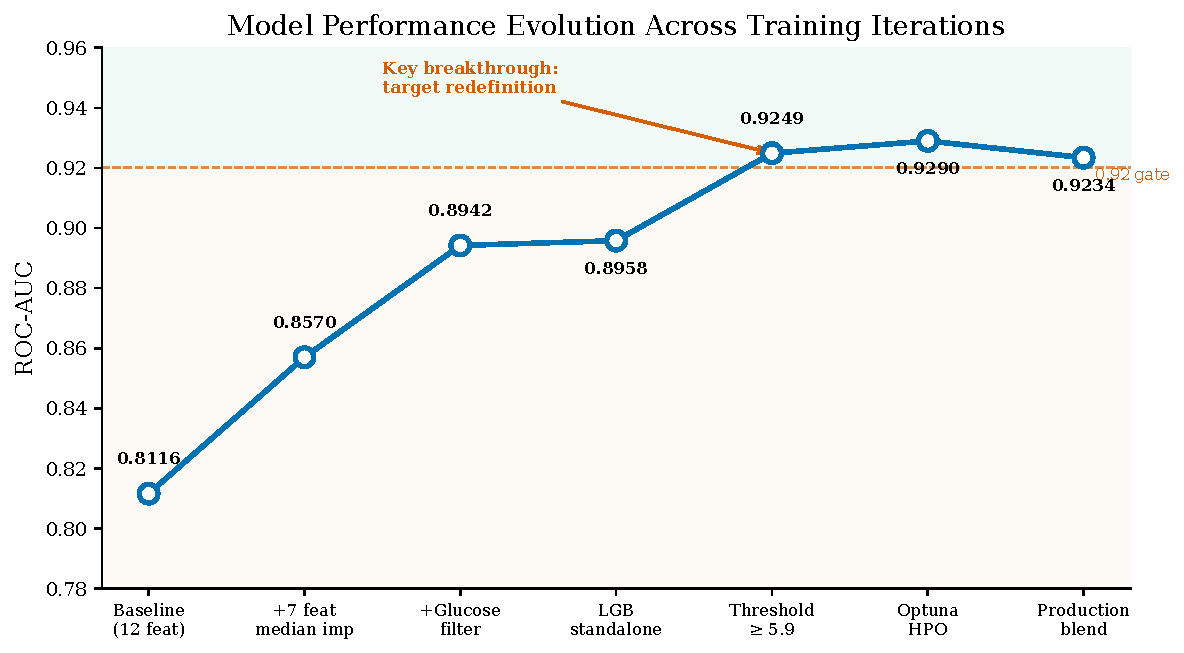
\includegraphics[width=\linewidth]{Assets/model_evolution.pdf}
\caption{Model evolution across seven iterative training rounds. The largest single AUC gain occurs at Round~5 when the target threshold is shifted from $\geq$5.7\% to $\geq$5.9\%, illustrating that threshold redefinition yielded the largest single-step AUC gain among all design changes.}
\label{fig:model_evolution}
\end{figure}

\subsection{Comparison with Related Work}

Table~IV contextualises the performance of the proposed system against comparable systems reported in the literature.

\begin{table}[htbp]
\caption{Comparison with Related Systems}
\label{tab:comparison}
\centering
\resizebox{\columnwidth}{!}{%
\begin{tabular}{llclcc}
\toprule
\textbf{System} & \textbf{Dataset} & \textbf{AUC} & \textbf{XAI} & \textbf{Multi-Thr.} & \textbf{Depl.} \\
\midrule
DRPM~\cite{b3} & NHANES & --- & No & No & No \\
CatBoost+Chat~\cite{b9} & 520 pts & --- & SHAP+Chatbot & No & No \\
Shah et al.~\cite{b7} & Public & 0.82 & SHAP, t-SNE & No & No \\
IMPACT~\cite{b11} & Multiple & --- & DiCE+LLM & No & No \\
ProxCF~\cite{b10} & PIDD & --- & Counterfactual & No & No \\
\textbf{Proposed ($\geq$5.9\%)} & \textbf{NHANES} & \textbf{0.923} & \textbf{SHAP+DiCE+WHO} & \textbf{Yes} & \textbf{Yes} \\
\textbf{Proposed ($\geq$6.5\%)} & \textbf{NHANES} & \textbf{0.972} & \textbf{SHAP+DiCE+WHO} & \textbf{Yes} & \textbf{Yes} \\
\bottomrule
\end{tabular}%
}
\vspace{2pt}

\raggedright\scriptsize `---' indicates AUC not reported for the diabetes prediction task in the original paper. `Proposed' refers to the system introduced in this work. Multi-Thr.\,=\,Multi-Threshold; Depl.\,=\,Deployment.
\end{table}

The proposed system achieves competitive to superior discriminative performance while providing the most comprehensive explainability stack among the compared systems. Unlike IMPACT~\cite{b11}, which combines counterfactuals with an LLM for multi-disease contexts, the proposed system integrates SHAP, DiCE, and epidemiological cross-validation within a unified diabetes-specific pipeline. The multi-threshold design provides a capability absent in all compared systems, enabling contextual adaptation without model retraining.

\subsection{Key Methodological Insights}

Three methodological insights emerged from this work. First, the removal of HbA1c from the feature set---despite its obvious predictive power---was essential for clinical validity. Replacing it with FastingGlucose required filtering to the NHANES fasting subsample (reducing the dataset from 67,876 to 33,333 records) but produced a model that genuinely learns risk patterns from non-target biomarkers, a prerequisite for real-world deployment where HbA1c is the unknown quantity being predicted. Second, the empirical superiority of median imputation over MICE for tree-based models is a noteworthy finding. MICE's iterative regression-based imputation creates synthetic inter-feature correlations that gradient-boosted trees exploit as genuine signal, producing inflated training metrics that do not generalise. Median imputation, combined with explicit missingness indicators, provides a more honest representation of the data's information content. Third, the weighted-blend ensemble matched or exceeded the stacking classifier while being approximately 5$\times$ faster to train, simpler to deploy, and more interpretable. The explicit blend weights provide immediate insight into which learner dominates for each threshold, facilitating clinical trust and debugging.

\subsection{Conclusion}

This paper presented a multi-threshold explainable ensemble framework for Type~2 diabetes risk prediction. The system addresses critical limitations in existing approaches through four primary contributions: (1)~a multi-threshold design that enables clinicians to select from three HbA1c thresholds ($\geq$5.7\%, $\geq$5.9\%, $\geq$6.5\%) tailored to their screening context; (2)~a threshold-effect ablation analysis demonstrating that threshold redefinition ($\geq$5.7\%$\rightarrow$$\geq$5.9\%: +0.029; $\geq$5.9\%$\rightarrow$$\geq$6.5\%: +0.047 AUC) yielded larger per-step improvements than four rounds of feature engineering, imputation, and model selection (+0.084 AUC combined), with final AUCs of 0.885, 0.923, and 0.972; (3)~a three-tier explainability framework integrating SHAP explanations, DiCE counterfactual interventions, and WHO epidemiological cross-validation; and (4)~a production-grade deployment architecture with fairness monitoring, HIPAA-compliant data handling, and containerised infrastructure. The principal methodological insights---that threshold redefinition yielded larger per-step AUC gains than model architecture changes, that median imputation outperforms MICE for tree-based ensembles, and that weighted blending matches stacking with superior practical properties---offer generalisable guidance for clinical ML practitioners.

Several limitations warrant acknowledgement. The reliance on NHANES data, while providing a large and representative U.S.\ population sample, may limit generalisability to non-U.S.\ populations with different dietary patterns, genetic predispositions, or healthcare access profiles. The system's predictive performance is inherently bounded by the information content of non-HbA1c clinical variables; the $\geq$5.7\% threshold's AUC plateau at 0.885 reflects a fundamental distributional limitation rather than a modelling deficiency. Additionally, while the WHO cross-validation provides ecological consistency, it does not constitute external clinical validation on independently collected patient cohorts.

%==============================================================================
% SECTION IV: FUTURE RESEARCH DIRECTION
%==============================================================================
\section{Future Research Direction}

Several promising research directions emerge from this work. First, external validation on clinical datasets from non-U.S.\ populations is essential to assess cross-cultural and cross-ethnic generalisability, particularly for regions with differing dietary patterns, genetic predispositions, and healthcare infrastructure profiles. Collaborations with international clinical centres would enable assessment of whether the multi-threshold framework and feature engineering strategies transfer effectively to populations beyond the NHANES demographic.

Second, the integration of longitudinal data from successive NHANES cycles presents an opportunity to model temporal risk trajectories rather than point-in-time predictions. Time-series modelling of glycaemic progression could enable personalised risk forecasts that capture the dynamic nature of diabetes development, potentially incorporating recurrent neural network or transformer architectures for sequential patient data~\cite{b14, b17}.

Third, the incorporation of agentic AI capabilities~\cite{b15, b16} represents a transformative future direction. Autonomous agents could orchestrate multi-step clinical workflows, including automated patient follow-up scheduling, adaptive intervention planning based on longitudinal risk monitoring, and intelligent triage decisions. Such agents would extend the proposed system from a prediction tool to an active clinical decision partner.

Fourth, integration with continuous glucose monitoring (CGM) systems using transformer-based deep learning~\cite{b17, b18} would enable real-time risk assessment for patients with wearable sensors. This hybrid approach---combining population-level survey data with individual-level continuous monitoring---could substantially improve predictive granularity and enable proactive interventions before glycaemic deterioration becomes clinically apparent.

Fifth, the counterfactual engine can be expanded through the integration of causal discovery methods~\cite{b6} to distinguish correlational from causal intervention pathways. Current counterfactual recommendations are based on predictive associations; incorporating causal inference would ensure that recommended lifestyle modifications are grounded in genuine causal relationships rather than statistical correlations.

Sixth, federated learning approaches offer a pathway to train models across multiple healthcare institutions without centralising sensitive patient data. This privacy-preserving methodology would expand the training dataset diversity while maintaining HIPAA compliance and institutional data governance requirements.

Finally, the development of personalised threshold selection algorithms---which recommend the optimal HbA1c threshold for each patient based on their clinical profile, comorbidities, and risk tolerance---would further enhance the clinical utility of the multi-threshold framework, moving from clinician-selected to data-driven threshold adaptation.

%==============================================================================
% REFERENCES
%==============================================================================
\begin{thebibliography}{00}

\bibitem{b1} P. B. Khokhar, C. Gravino, and F. Palomba, ``Advances in artificial intelligence for diabetes prediction: Insights from a systematic literature review,'' \textit{Artificial Intelligence in Medicine}, vol.~164, p.~103132, 2025.

\bibitem{b2} M. Khalifa and M. Albadawy, ``Artificial intelligence for diabetes: Enhancing prevention, diagnosis, and effective management,'' \textit{Computer Methods and Programs in Biomedicine Update}, 2024.

\bibitem{b3} F. Nie, X. Song, and W. Chen, ``DRPM: An advanced predictive model for early diabetes detection and risk stratification,'' \textit{Heliyon}, 2024.

\bibitem{b4} S. S. Bontha, S. K. R. Jammalamadaka, C. P. Vudatha, S. B. Jammalamadaka, B. K. Duvvuri, and B. C. Vudatha, ``Predicting risk and complications of diabetes through built-in artificial intelligence,'' \textit{Applied Sciences}, 2024.

\bibitem{b5} I. Tasin, T. U. Nabil, S. Islam, and R. Khan, ``Diabetes prediction using machine learning and explainable AI techniques,'' \textit{Healthcare Technology Letters}, vol.~10, no.~1--2, pp.~1--10, 2023.

\bibitem{b6} M. J. Noh and Y. S. Kim, ``Diabetes prediction through linkage of causal discovery and inference model with machine learning models,'' \textit{Applied Sciences}, 2024.

\bibitem{b7} P. Shah, M. Shukla, N. H. Dholakia, and H. Gupta, ``Predicting cardiovascular risk with hybrid ensemble learning and explainable AI,'' \textit{Scientific Reports}, 2025.

\bibitem{b8} S. S. Prakash and A. C. Subhajini, ``An efficient prediction and analysis of diabetics based on hybrid convolutional pyramid squeeze attention network with explainable AI,'' \textit{International Journal of Pattern Recognition and Artificial Intelligence}, vol.~39, no.~12, p.~2557012, 2025.

\bibitem{b9} E. Maimaitijiang, M. Aihaiti, and Y. Mamatjan, ``An explainable AI framework for online diabetes risk prediction with a personalized chatbot assistant,'' \textit{Healthcare Analytics}, 2025.

\bibitem{b10} M. F. Kabir, A. M. Mahakal, Y. Wang, A. AlSobeh, B. Al-Ahmad, and R. S. Alkhawaldah, ``Proximity-constrained counterfactuals for explainable diabetes risk assessment,'' \textit{Applied Computational Intelligence and Soft Computing}, vol.~2025, p.~3424976, 2025.

\bibitem{b11} P. K. Mohanty, S. A. J. Francis, R. K. Barik, K. H. K. Reddy, D. S. Roy, and M. J. Saikia, ``IMPACT: An interactive multi-disease prevention and counterfactual treatment system using explainable AI and a multimodal LLM,'' \textit{PeerJ Computer Science}, 2025.

\bibitem{b12} J. Prashanthan and A. Prashanthan, ``Predicting the future risk of developing type 2 diabetes in women with a history of gestational diabetes mellitus using machine learning and explainable artificial intelligence,'' \textit{Primary Care Diabetes}, vol.~19, pp.~658--666, 2025.

\bibitem{b13} M. Aljaafari, S. E. El-Deep, A. A. Abohany, and S. E. Sorour, ``Integrating innovation in healthcare: The evolution of CURA's AI-driven virtual wards for enhanced diabetes and kidney disease monitoring,'' \textit{IEEE Access}, vol.~12, pp.~128045--128067, 2024.

\bibitem{b14} R. Esmaeilyfard and M. Bayati, ``Enhancing AI-driven forecasting of diabetes burden: A comparative analysis of deep learning and statistical models,'' \textit{Scientific Reports}, vol.~15, 2025.

\bibitem{b15} D. B. Acharya, K. Kuppan, and B. Divya, ``Agentic AI: Autonomous intelligence for complex goals---A comprehensive survey,'' \textit{IEEE Access}, vol.~13, pp.~17535--17555, 2025.

\bibitem{b16} S. Hosseini and H. Seilani, ``The role of agentic AI in shaping a smart future: A systematic review,'' \textit{Array}, vol.~26, p.~100399, 2025.

\bibitem{b17} Y. Lu, D. Liu, Z. Liang, R. Liu, Y. Liu, J. Li, Z. Feng, P. Chen, L. M. Li, B. Sheng, W. Jia, L. Chen, H. Li, and Y. Wang, ``A pretrained transformer model for decoding individual glucose dynamics from continuous glucose monitoring data,'' \textit{National Science Review}, vol.~12, p.~nwaf039, 2025.

\bibitem{b18} T. Zhu, L. Kuang, C. Piao, J. Zeng, K. Li, and P. Georgiou, ``Population-specific glucose prediction in diabetes care with transformer-based deep learning on the edge,'' \textit{IEEE Transactions on Biomedical Circuits and Systems}, vol.~18, no.~2, pp.~236--246, 2024.

\end{thebibliography}

\end{document}
